\section{Architecture}
\thispagestyle{plain}

The current architecture of the application is as shown in the figure 1 from the requirements-section. We have a back-end written in Java that retrieves information from services like Digitalt Fortalt, Flickr and Instagram. Digitalt Fortalt is where all the stories are obtained from, Flicker holds all the locations, and the pictures are taken from Instagram based on tags. The information is stored on the server and can now be used by the client, which holds the front-end of the application that is being developed on Appcelerator Titanium, using mainly JavaScript and XML. Twitter is integrated directly into the front-end and does not have to go through the server. This is what we eventually would like to do for all the external services, and completely get rid of the back-end, but given the time available for the project and the features the customer wants us to implement, this is not a task that will be developed. We would also like the user to be able to publish to more of the external services via the application. Publish a picture to Instagram, add a new location to Flickr, or share a story on Facebook are all features we would like to add, but are not top priority given our time restrictions.

\subsection{Backend}
The Back-end is written in Java and mainly retrieves data from external APIs and save it on the server so that it can be used by the application.

\begin{figure}[!h]
\begin{center}
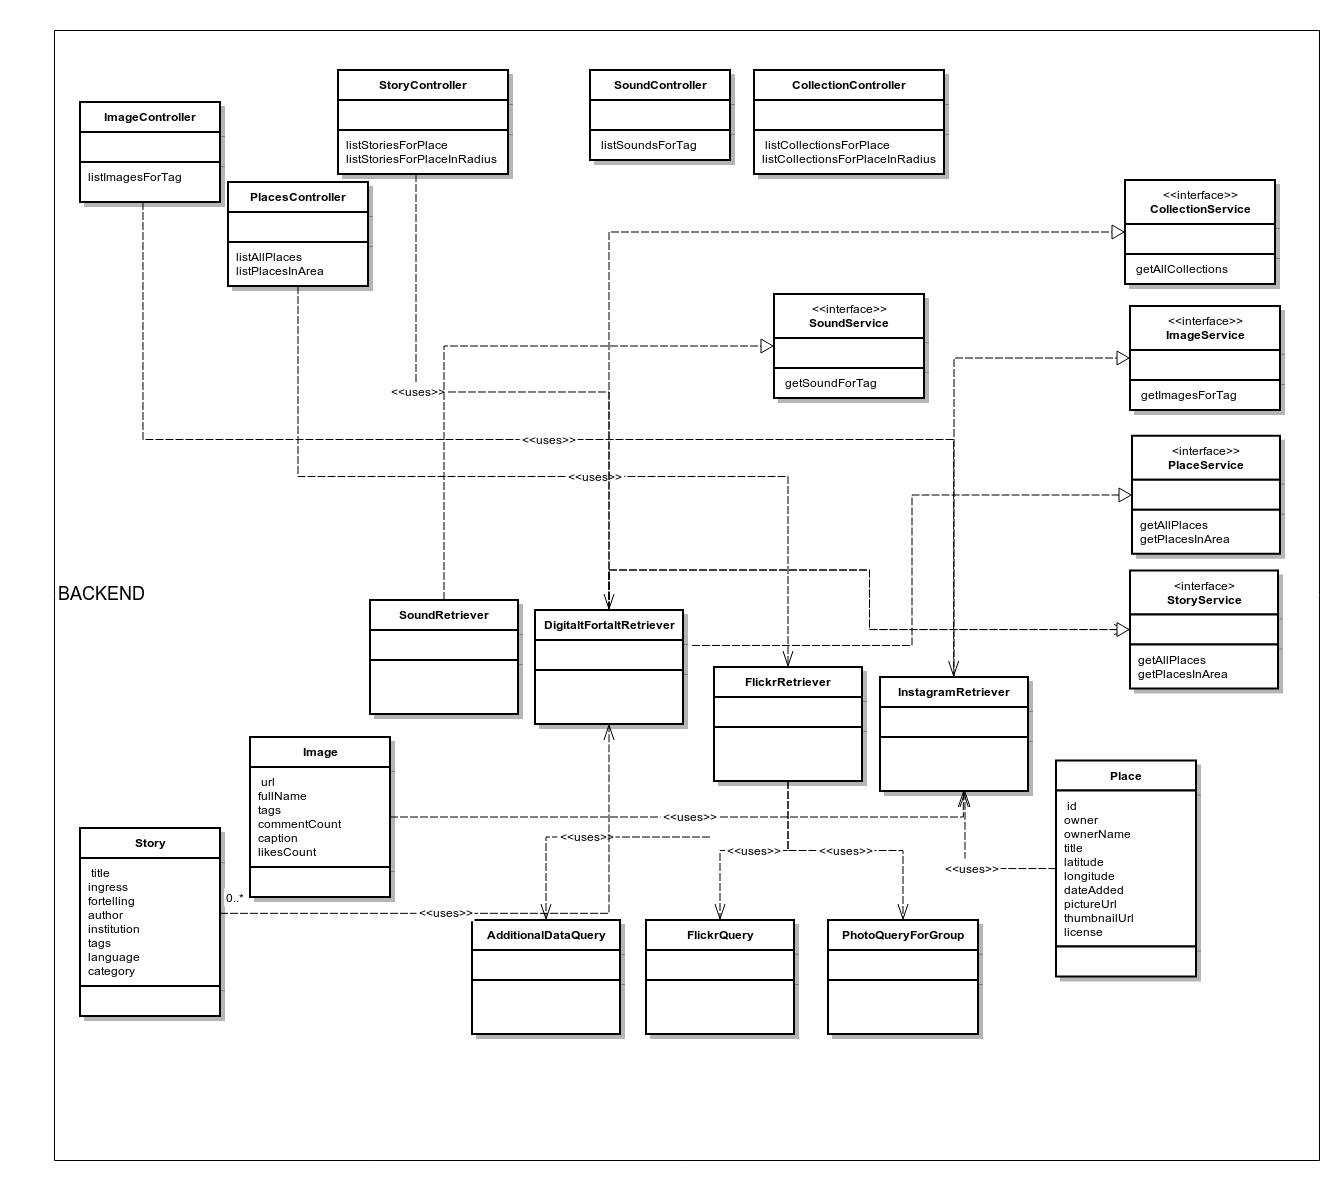
\includegraphics[scale=0.1]{class-backend.jpg}
\caption{Back-end (Full scale can be found in Attachments) }
\end{center}
\end{figure}

\subsection{Frontend}
The front-end of the application is an interface to let the user enter, manipulate and view data. It is the part of the application that is being interpreted on the users own device, and is based on XML, TSS and JavaScript for design and functionality. 

Every window in the application has a JavaScript-, TSS- and XMLl-file associated with it. A window can contain various views that can each have different event listeners. What the user sees depends on the window currently open and its associated XML, TSS and JavaScript files and what happens when interacting with a view depends on the event-listeners attached to that particular view. Interactions can be purely visual or it can trigger core functionalities. For example the refresh button on the map window has an event-listener attached to it so that when the user clicks it, it will attempt to fetch the locations from the server and plot them on the map. It will also animate the refresh icon to spin, giving the user feedback that the click was registered.

\begin{figure}[!h]
\begin{center}
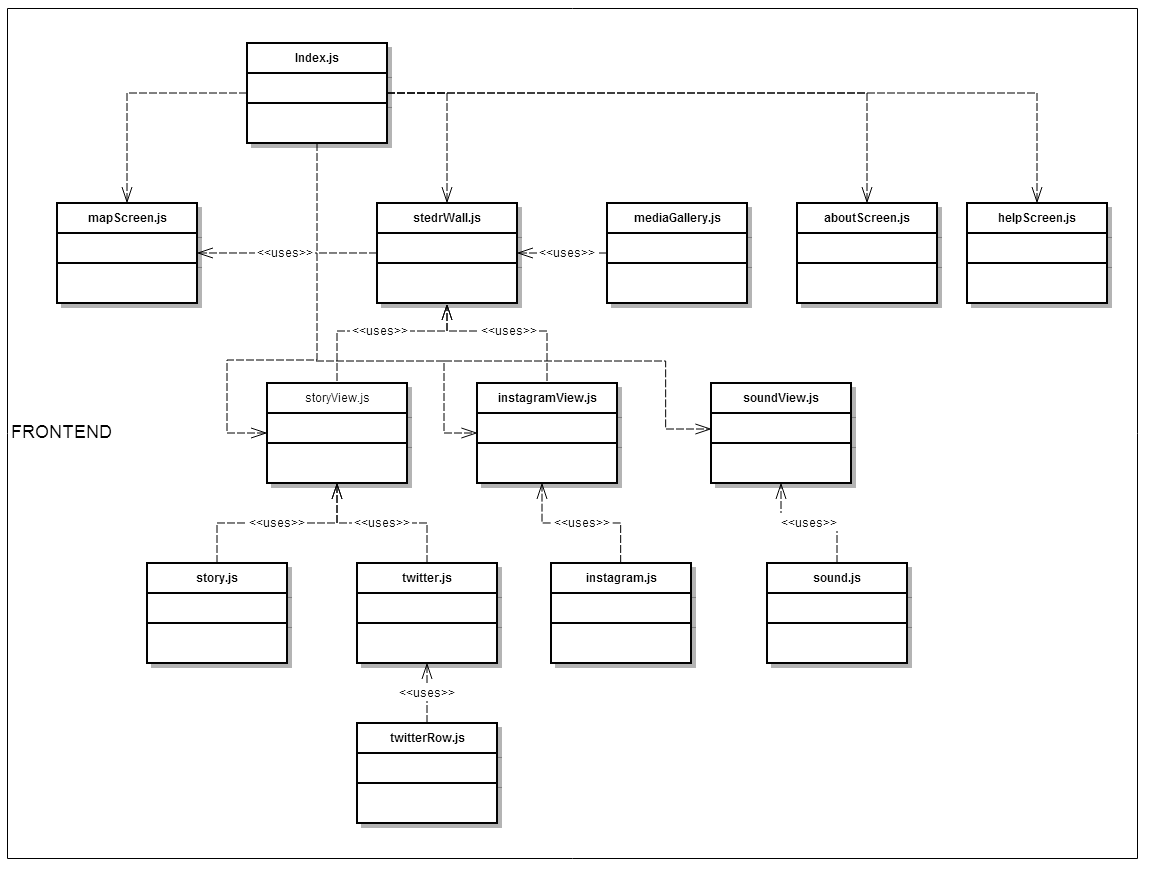
\includegraphics[scale=0.1]{class-frontend.png}
\caption{Front-end (Full scale can be found in Attachments)}
\end{center}
\end{figure}

\subsection{Use Case}

\begin{figure}[!h]
\begin{center}
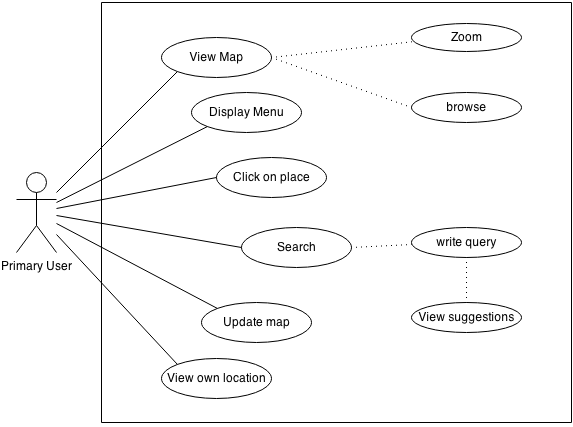
\includegraphics[scale=0.6]{ms.png}
\caption{Map View (Home)}
\end{center}
\end{figure}

\begin{figure}[!h]
\begin{center}
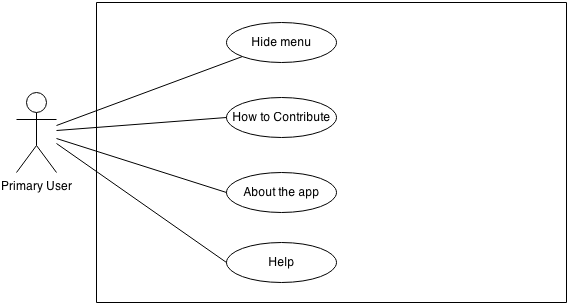
\includegraphics[scale=0.6]{mens.png}
\caption{Menu View}
\end{center}
\end{figure}

\begin{figure}[!h]
\begin{center}
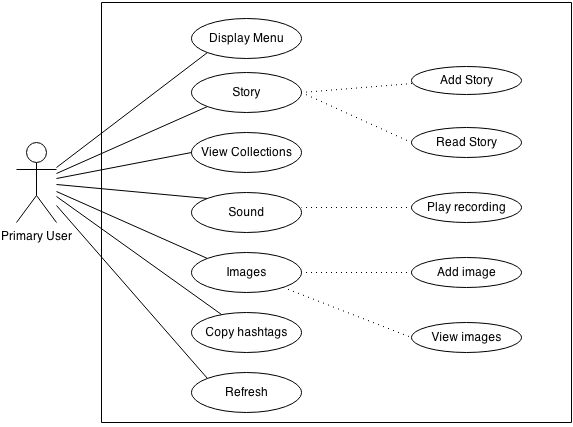
\includegraphics[scale=0.6]{ps2.png}
\caption{Place Screen}
\end{center}
\end{figure}

\clearpage

\subsection{Sequence}

\begin{figure}[!h]
\begin{center}
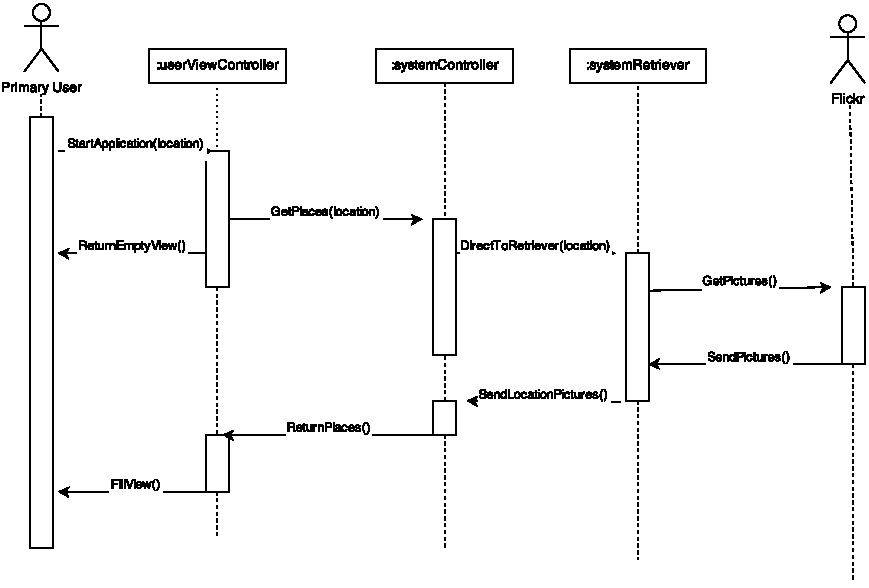
\includegraphics[scale=1]{Get-Stories}
\caption{Get Stories}
\end{center}
\end{figure}

\begin{figure}[!h]
\begin{center}
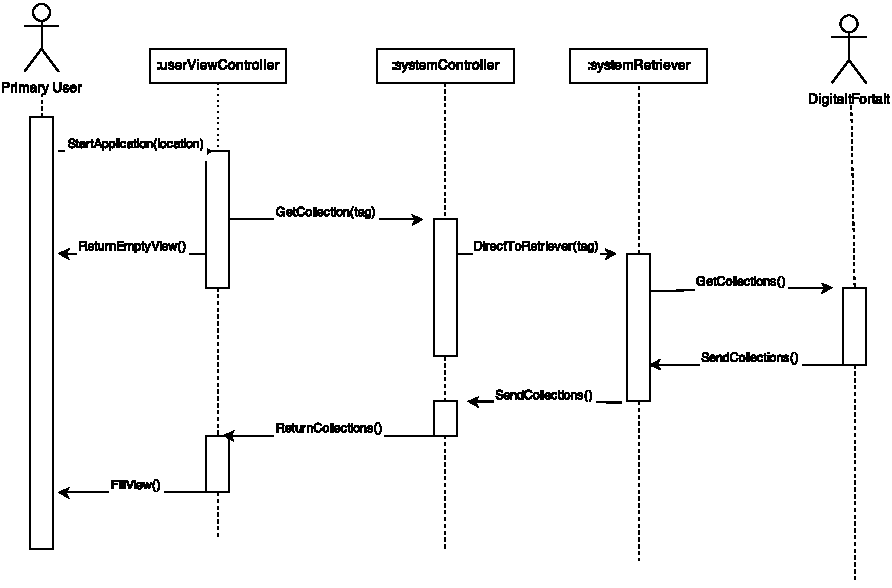
\includegraphics[scale=1]{Get-Collections}
\caption{Get Collections}
\end{center}
\end{figure}